\documentclass[12pt]{article}
%\usepackage{amsmath}
\usepackage{graphicx}
%\usepackage{enumerate}
\usepackage{natbib} %comment out if you do not have the package
\usepackage{url} % not crucial - just used below for the URL 
\usepackage{amsmath, amssymb}
\usepackage[top=1.25in]{geometry}


%\pdfminorversion=4
% NOTE: To produce blinded version, replace "0" with "1" below.
\newcommand{\blind}{0}

% DON'T change margins - should be 1 inch all around.
\addtolength{\oddsidemargin}{-.5in}%
\addtolength{\evensidemargin}{-.5in}%
\addtolength{\textwidth}{1in}%
\addtolength{\textheight}{1.3in}%
\addtolength{\topmargin}{-.8in}%


\begin{document}

%\bibliographystyle{natbib}

\def\spacingset#1{\renewcommand{\baselinestretch}%
{#1}\small\normalsize} \spacingset{1}


%%%%%%%%%%%%%%%%%%%%%%%%%%%%%%%%%%%%%%%%%%%%%%%%%%%%%%%%%%%%%%%%%%%%%%%%%%%%%%

\if0\blind
{
\vspace{-1cm}
  \title{\bf Coupling material and mechanical design processes via computer model calibration}
  \author{Carl Ehrett\hspace{.2cm}\\
    School of Mathematical and Statistical Sciences, Clemson University,\\
    D. Andrew Brown \\
    School of Mathematical and Statistical Sciences, Clemson University,\\
    Evan Chodora \\
    Department of Mechanical Engineering, Clemson University,\\
    Mingzhe Jiang \\
    Department of Chemical and Biomolecular Engineering, Clemson University,\\
    Christopher Kitchens \\
    Department of Chemical and Biomolecular Engineering, Clemson University,\\
    and\\
    Sez Atamturktur \\
    Department of Architectural Engineering, Pennsylvania State University\\}
  \maketitle
} \fi

\if1\blind
{
  \bigskip
  \begin{center}
    {\LARGE\bf Title}
\end{center}
  \medskip
} \fi

\begin{abstract}
In traditional engineering design, material selection is a matter of choosing a material with appropriate properties for the project at hand from a database of known materials, often as a matter of ad-hoc satisficing. 
%
Material design usually occurs separately, and without an eye to specific end-uses. 
%
It is desirable to wed these design processes, selecting a material design by modeling its performance outcomes in a particular engineering application. 
%
Therefore, here we offer an example of calibrating material design parameters to desired performance targets for a wind turbine blade. 
%
%A well-established framework for the calibration of computer models is provided by \cite{Kennedy2001} and the myriad works that build upon it. 
%%
%Common to those approaches is the assumption that calibration is a matter of estimating unknown and/or uncontrollable parameters by attuning the model to data obtained through physical experimentation. 
%%
%In this work we seek to find optimal settings for the design of a composite material for use in a wind turbine blade.
%
We show that existing techniques for model calibration can be profitably reconceptualized as a method for optimization and applied to solve this material design problem.
%In order to find optimal settings for the design of a composite material for use in a wind turbine blade, we apply techniques for model calibration as a method for optimization.
%
Rather than calibrating a model to find a posterior distribution of unknown parameters in order to bring the model maximally into agreement with reality, we calibrate to find a posterior distribution on controllable model inputs in order to bring the predicted system behavior into agreement with pre-determined performance targets. 
%
In essence, we treat performance targets as ``desired observations'' and use them as the data in the calibration problem. 
%
We demonstrate our proposed methodology in both an artificial case and in the case of a finite element model of wind turbine blade performance and cost. 
%
In the latter case, we demonstrate how to estimate the Pareto front with uncertainty bands. 
\end{abstract}

\noindent%
{\it Keywords:}  Gaussian processes, material design, optimization, Pareto optimality, Uncertainty quantification, wind turbines
\vfill



\end{document}


%Generalizing from \cite{Kennedy2006}, I expand the Bayesian analysis to include the diagonal observation variance matrix $\mathbf C_{\mathbf y}$, rather than requiring this value to be specified as known, and I allow for a non-uniform prior $\pi(\boldsymbol \theta)$ on the calibration parameters. By (\ref{eq:full_dist}) on page \pageref{eq:full_dist}, 
%since I estimate $\boldsymbol \rho^\eta,\lambda_\eta$ by maximum likelihood, set $c=0$, and do not include a discrepancy function, we have for desired observations $\mathbf y=(y (b_{n+1}),\cdots,y(b_{n+m}))^T$ and $\mathcal D=(\mathbf y^T, \boldsymbol\eta^T)^T$:
%\begin{equation}\label{eq:the_model}
%\pi(\boldsymbol \theta,\mathbf C_{\mathbf y}|\mathcal D) \propto \pi (\mathcal D|\boldsymbol \theta,\mathbf C_{\mathbf y})\times \pi(\boldsymbol \theta)\times \pi(\mathbf C_{\mathbf y})
%\end{equation}
%and $\mathcal D|\boldsymbol \theta,\mathbf C_{\mathbf y} \sim N(\boldsymbol 0_{m+n}, \mathbf C_{\mathcal D})$, 
%\begin{equation}\label{eq:the_covariance}
%\mathbf C_{\mathcal D} = \mathbf C_{\boldsymbol\eta} + 
%\begin{bmatrix}
%\mathbf C_{\mathbf y} & \boldsymbol 0\\ 
%\boldsymbol 0 & \boldsymbol 0
%\end{bmatrix}
%\end{equation}
%where $\mathbf C_{\boldsymbol\eta}$ is a $(m+n)\times(m+n)$ matrix with $i,j$ entry $C(b_i,b_j)$.
%
%The model as described above leaves open several details of the model, options for which are explored in the remainder of Section \ref{MCMC}. In \ref{des_obs_var} I consider options for $\pi(\mathbf C_{\mathbf y})$, the prior on observation variance, including setting a degenerate prior corresponding to specifying a known observation variance. In \ref{which_data} I take up the question of which data one ought to desire, showing how the goals of one's analysis can support vastly different choices for desired data. In \ref{removing_cal_pars} I explore options for $\pi(\boldsymbol \theta)$, the prior on the calibration parameters. I depart thereby from the framework of \cite{Kennedy2006}, who (implicitly) restrict the calibration model to the case of using a uniform prior. An example is used to show how setting a non-uniform prior here can allow one to reduce the number of parameters that are subjected to calibration in the model. Before taking up these matters, in \ref{convergence_difficulties} I take up convergence difficulties that arise due to boundary constraints on the calibration parameters.
%\subsubsection{Full model and likelihood}
%Blah
%
%\subsection{Convergence difficulties}\label{convergence_difficulties}
%% And the idea to eliminate boundary constraints
%As will often be the case in calibration problems, in the application considered here the calibration parameters $(v,k)$ have compact support: $v\in [.1,.6],$ $k\in [10\mathrm{mm},25\mathrm{mm}]$.
%%DISCUSS Andrew asks "Is compact support necessary? For the sake of posterior inference, it seems to me that one could do just as well with open parameter sets." I'm not sure what he means: is he suggesting that reparameterization to open sets is possible? Or that ignoring the boundaries is? Or something else? And either way, how does it affect the point made here?
%When the calibration procedure leads to draws near these boundaries, the MCMC routine may suffer poor mixing. For example, consider using proposal density $q$ such that $(v^*,k^*)\sim N((v^{(i)},k^{(i)}),\Sigma)$ for some proposal covariance $\Sigma$. 
%The symmetry of a normal proposal density makes it convenient for MCMC, but also exacerbates the difficulties that come from boundary conditions. 
%Using such a proposal density with $\pi(\boldsymbol \theta)$ a uniform density on the support of $\boldsymbol \theta$ amounts to simply discarding any proposed draw of $(v,k)$ that falls outside of the boundaries for those variables. 
%This is inefficient, as it leads to low acceptance rates during MCMC for new draws of $\boldsymbol \theta$. 
%When a new proposed draw is rejected, the previous draw is repeated, leading to extremely high levels of autocorrelation in the MCMC draws.
%
%%DISCUSS What are some sources for reflecting boundary proposals?
%
%There are several ways to tackle this problem. 
%One approach seeks to improve acceptance rates through utilizing an adaptive proposal covariance magnitude, so that $\Sigma$ is periodically updated during the burn-in period in order to achieve an optimal acceptance ratio of around 23\%; see \cite{Roberts1997}. 
%If $\Sigma$ is diagonal, then this is especially simple to implement. 
%One simply keeps track of the number of times that a proposed draw of $\theta_i$ is outside of its boundaries, and then every 100 MCMC steps or so, if the number of out-of-boundary proposals exceeds a specified threshold, then one reduces $\Sigma_i$, the proposal variance of $\theta_i$. 
%This strategy can easily be paired with a more comprehensive adapative proposal covariance -- e.g., one that is set to increase in magnitude whenever more than 30 of the most recent 100 draws have been accepted, and decrease in magnitude whenever fewer than 20 of the most recent draws have been accepted. 
%If the posterior distribution is merely near the boundary, such measures may suffice; however, in calibration to desired observations (which tend to be extreme outliers \textit{qua} observations), often the calibration parameters will be drawn strongly to the boundaries, and in such a situation the sort of adaptive proposal distribution described above may be insufficient to secure good acceptance ratios. 
%
%A second strategy is to use an independence chain approach \citep{Tierney1994}, in which the proposal density is independent of all previous draws. E.g., for compact support $\mathcal S$, one could simply draw new proposals as uniform over $\mathcal S$. When the posterior distribution is diffuse over its support, this can be effective. Otherwise, it can lead to low acceptance rates, as too many proposals are generated in low-density areas of the posterior distribution. 
%
%A third strategy would be to transform the variables to be unbounded. This requires describing the model in terms of these transformed variables. An adaptive covariance can be used here as well, further improving acceptance rates. A fourth, closely related strategy would be to employ some variety of proposal with the same support as the variables. Indeed, the difference between the third and fourth strategies is largely conceptual. Consider, for example, using the logit transform to remove boundary constraints from variables with compact support. Without boundary constraints, one can recover the convenience of a symmetric, Gaussian proposal distribution, without risk of proposing outside of the variables' support. But in addition to being viewed as a symmetric distribution on the transformed variables, this can equally be viewed as a non-symmetric distribution on the untransformed variables. I apply this logit transform to $(v,k)$ in the wind turbine application, where for convenience I adopt the latter conceptual perspective. 
%
%The adaptive proposal strategy sketched above changes only the magnitude of the proposal covariance, and depends upon having a diagonal covariance matrix. This diagonality is what allows the easy modification of the magnitude of the variance of all and only those parameters which are being drawn outside of their boundary constraints. But where boundary constraints are no longer a problem, it is just as convenient to establish a non-diagonal proposal covariance. This will, of course, be of especially high value when the calibration parameters are correlated in the posterior distribution, which is frequently the case. Thus, when updating the proposal covariance, one can set it to be equal to the sample covariance of the unique samples accepted thus far in the MCMC routine.
%
%%In the case of compact support, using the logit transform on the normalized variable removes the boundary constraints. Without boundary constraints, one can recover the convenience of a symmetric proposal, such as a normal distribution. An adaptive proposal covariance further aids strong mixing here. The adaptive proposal strategy sketched above depends upon having a diagonal proposal covariance matrix for the calibration parameters; this is what allows the easy modification of the magnitude of the variance of all and only those parameters which are being drawn outside of their boundary constraints. But where boundary constraints are no longer a problem, it is just as convenient to establish a non-diagonal proposal covariance. This will, of course, be of especially high value when the calibration parameters are correlated in the posterior distribution, which is frequently the case in our application. Thus, when updating the proposal covariance, one can set it to be equal to the sample covariance of the unique samples accepted thus far in the MCMC routine. 
%
%
%If the acceptance ratio is low early in the MCMC when using this adaptive technique, the resulting proposal covariance may be too small. To promote more efficient exploration of the parameter space, the covariance can be multiplied by a constant $\tau$ which is also updated whenever the proposal covariance is updated. One may adjust $\tau$ so as to induce acceptance rates close to 23\%. Thus, during the burn-in period, every $n_0$ draws (with $n_0$ set to, e.g., 100), the proposal covariance $\Sigma$ and multiplier $\tau$ are updated to $\Sigma^*$ and $\tau^*$ as follows, where $a$ is the proportion of the past $n_0$ draws that were accepted, $I$ is the indicator function, and $\mathbf S$ is the set of all samples drawn so far:
%\begin{equation}
%\begin{aligned}
%\tau^* &= \tau \cdot (1.25  I(a>25) + 0.75 I(a<20))\\
%\Sigma^* &= \tau^* \cdot \mathrm{Cov}(\mathbf S)
%\end{aligned}
%\end{equation}
%
%%More cautiously (lest the proposal covariance become unduly influenced by early, nonrepresentative draws) but in the same spirit, one can proceed as follows. Set the proposal covariance to begin as some pre-specified, diffuse covariance (such as the identity $I$). Periodically update to a weighted mixture of the previous covariance matrix with the sample covariance of the most recent 50\% of the unique samples drawn in the MCMC routine, where the weight increases to favor the sample covariance over the course of the burn-in period. Furthermore, a scalar multiplier $\tau$ of the proposal covariance can be adjusted so as to induce acceptance rates close to 23\%. This strategy was found to be most successful in our application. Thus where the first $g$ samples are treated as burn-in, each time the proposal covariance $\Sigma$ and multiplier $\tau$ are updated to $\Sigma^*$ and $\tau^*$ at the $r^{\text{th} }$ iteration:
%%\begin{equation}
%%\tau^* =  \tau \left ( 0.9 \cdot I(a<0.2) + 1.1 \cdot I(a>0.3)\right),\quad
%%\Sigma^* = \tau^* \left (  
%%\frac{g-r}\rho \Sigma + \frac r g C_U \right)
%%\end{equation}
%%where $I(\cdot)$ is the indicator function, $a$ is the acceptance rate from recent (e.g. previous 100) draws, and $C_U$ is the sample covariance of the most recent half of all unique samples drawn in the MCMC routine.
%
%The adaptation takes place only during the burn-in period. 
%As a result, the adaptive nature of the algorithm does not change the fact that it is an implementation of the Metropolis-Hastings algorithm given in \cite{Hastings1970}. Hence it is guaranteed to converge to the target distribution. 
%However, another option would be to employ the adaptive Metropolis schema of \cite{Haario2001,Haario2005,Haario2006}, who continue to update the proposal covariance to be the sample covariance of all previous draws throughout the sampling procedure (up to a scaling constant which, unlike $\tau$ above, is not itself adaptive). This sampling method loses the Markov property and hence is not an MCMC method. 
%Nonetheless the authors show it is ergodic under the conditions that the target distribution is bounded with bounded support. 
%
%Recall (from Section \ref{MCMC_methods}) that abandoning symmetry in one's proposal distribution requires that one employ the more general Metropolis-Hastings algorithm, rather than the Metropolis algorithm of \cite{Metropolis1953}. Interpreting a normal distribution on the logit-transformed variables as a distribution on the original variables, it is not symmetric. Therefore, calculate the log acceptance probability a proposal for the $i^{\text{th}}$ draw of $\boldsymbol \theta$ as 
%\begin{equation}
%\log \alpha = \log(\boldsymbol \theta^*|\mathcal D, \mathbf C_{\mathbf y}) - \log(\boldsymbol \theta^{(i-1)}|\mathcal D,\mathbf C_{\mathbf y}) + \log q(\boldsymbol \theta^{(i-1)}|\boldsymbol \theta^*)
%- \log q(\theta^* |\boldsymbol \theta^{(i-1)})
%\end{equation}
%where the use of the log scale is required in order to avoid significant round-off and underflow errors due to the dimensionality of $\mathcal D$.
%
%The benefits of the logit-transformed, unbounded proposal over a version of the MCMC using a normal proposal (with adaptive covariance) over the untransformed calibration parameters are displayed in Figure \ref{ACFs}. Sizeable autocorrelation appears in the untransformed version, whereas in the logit-transformed version the autocorrelation drops off to insignificance within about 30 steps.
%
%\begin{figure}
%\centering
%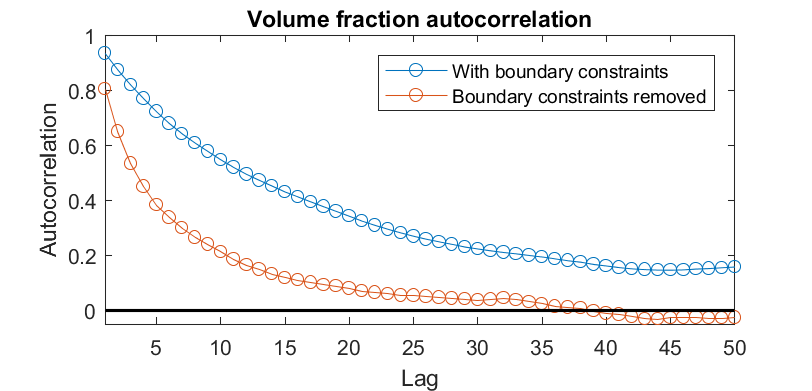
\includegraphics[width=.65\linewidth]{ACF_bnd_cnds_fig}
%\captionsetup{width=.65\linewidth}
%\caption{Auto-correlation for draws both with and without the elimination of boundary conditions.}
%\label{ACFs}
%\end{figure}

%\subsection{Desired observation variance}\label{des_obs_var}
%% 4 versions: heterosked constant, homosked constant, heterosked prior, homosked prior
%In the framework of \cite{Kennedy2006} on which much of the current approach is based, observation variance is assumed to be known. 
%That assumption is less straightforward in the case of CDO. 
%However, as explained below, there are applications in which setting a ``known'' observation variance is appropriate. 
%In this section, I consider the option of specifying observation variance versus setting a (non-degenerate) prior on observation variance. 
%I also consider the option of whether to set different observation variances for different outputs, or a single observation variance on all (standardized) outputs. 
%Table \ref{table:obs_vvar_comp} and the corresponding Figure \ref{fig:comp_obs_var} of MCMC results show how impactful are the choices amongst these options in the wind turbine blade design application. 
%The posterior mean model output varies significantly across the four available strategies, which correspond to different specifications of observation variance settings. 
%The table reflects the choices of (1) whether to specify that the observations are homoskedastic with respect to output type (e.g., whether standardized cost output has the same observation variance as standardized deflection output), and (2) whether the observation variance is set to a constant level or given a (nondegenerate) prior.
%From \eqref{eq:the_model} above, the full models corresponding to these choices, assuming a uniform prior on the calibration parameters, are as follows. 
%Columns one and two of the table both correspond to specifying $\boldsymbol \sigma = (\sigma^2_1,\sigma^2_2,\sigma^2_3)^T$ as the observation variance for each of the three outputs. 
%The two columns differ only in the value of $\boldsymbol \sigma$. 
%The prior $\pi(\mathbf C_{\mathbf y})$ in \eqref{eq:the_model} is thus the degenerate prior $\delta_{\boldsymbol\sigma}(\cdot)$, the Dirac delta function centered at $\boldsymbol \sigma$. 
%Here, $\mathbf C_{\mathbf y}$ is a diagonal matrix where the $i,i$ entry is equal to $\sigma^2_j$ iff desired observation $y_i$ is an observation of output $j$. 
%E.g., if $y_4$ is an observation of rotation, then the fourth diagonal element of $\mathbf C_{\mathbf y}$ is $\sigma^2_2$, the observation variance for rotation. 
%So for these two columns the full model is given by:
%\begin{equation}\label{eq:full_model_1}
%\begin{aligned}
%\pi(\boldsymbol\theta,\mathbf C_{\mathbf y}|\mathcal D) &\propto \pi(\mathcal D|\boldsymbol\theta,\mathbf C_{\mathbf y}) \times \pi(\boldsymbol\theta) \times \pi(\mathbf C_{\mathbf y})\\
%&\propto \pi(\mathcal D|\boldsymbol\theta,\mathbf C_{\mathbf y}) \\
%&\propto \lvert \mathbf C_{\mathcal D} \rvert ^{-1/2} \mathrm{exp}(\mathcal D^T \mathbf C_{\mathcal D}^{-1} \mathcal D)
%\end{aligned}
%\end{equation}
%where $\mathbf C_{\mathcal D}$ is given in \eqref{eq:the_covariance}, and where in the final expression I do not explicitly include the uniform $\pi(\boldsymbol\theta)$ or the degenerate $\pi(\mathbf C_{\mathbf y})$.
%Columns three and four each place a prior distribution on the observation variances. Column three places independent priors $1/\sigma^2_i$ on each of the $\sigma^2_i$, $i=1,2,3$, which serve as the observation variances of the three outputs. Column four places a single prior $1/\sigma^2_1$ on a scalar value $\sigma^2_1$ which serves as the observation variance for each of the three outputs. Thus the full models for these columns are:
%\begin{equation}\label{eq:full_model_2}
%\begin{aligned}
%\pi(\boldsymbol\theta,\mathbf C_{\mathbf y}|\mathcal D ) &\propto
%\pi(\mathcal D|\boldsymbol\theta,\mathbf C_{\mathbf y}) \times \pi(\boldsymbol\theta) \times \pi(\mathbf C_{\mathbf y})\\
%&\propto  \pi(\mathcal D|\boldsymbol\theta,\mathbf C_{\mathbf y}) \times \pi(\mathbf C_{\mathbf y})\\
%&\propto \lvert \mathbf C_{\mathcal D} \rvert ^{-1/2} \mathrm{exp}(\mathcal D^T \mathbf C_{\mathcal D}^{-1} \mathcal D) \times \prod_{i=1}^k \frac1{\sigma^2_i}
%\end{aligned}
%\end{equation}
%where for column three $k=3$ and $\mathbf C_{\mathbf y}$ is defined as in columns one and two, and for column four $k=1$ and $\mathbf C_{\mathbf y}=\sigma^2_1 \mathbf I_{m\times m}$. In both cases, the final expression does not explicitly include the uniform $\pi(\boldsymbol\theta)$.
%
%Notice in Table \ref{table:obs_vvar_comp} that column three is noticeably distinct from the others. Here is the only case in which the MCMC is free to alter the \emph{proportions} of observation variance allotted to the various outputs. In this case, the desired observation was essentially achieved for deflection and rotation, whereas the posterior cost was far from the desired cost. Thus, using the settings reflected in column three, we are able to learn that it is ``easier'' to achieve these two performance metrics than to achieve the cost target.
%
%When CDO is used without a discrepancy function and with observation variance sampled under a prior, the posterior distribution on observation variance amounts to an indirect measure of how closely reality can approximate our desired observations. E.g., from the fact that posterior observation variance from the routine represented in column three of Table \ref{table:obs_vvar_comp} was near zero, we see immediately that the cost target was achieved. Likewise, extremely high posterior observation variance indicates that the target could not be achieved. The posterior distribution reflects the (false) assumption that the difference between the desired observations and the true system mean is accounted for by random, mean-zero noise. 
%
%Matters are different when a set observation variance is specified for each output. Clearly, since the observation variance isn't sampled in the MCMC, there is no Bayesian learning to be had here. However, there is an opportunity to specify priorities through the specification of the variance. When the desired observations are outside the range of what is realistically achievable, the specific level of the observation variance is unlikely to matter much (unless it is so low as to engender computational difficulties). More important (in the case of multivariate output) is the fact that in specifying the observation variance, one is implicitly specifying the relative importance of each output. E.g., if I set a very diffuse observation variance on cost, and a very small one on deflection, then I have told the model that reduction in deflection is to be prioritized over reduction in cost. Whether one chooses to do so will depend on one's goals in calibration, as well as one's level of prior knowledge as to how close to reality one's desired observations are.
%
%Such prioritization can be harnessed to achieve calibration goals in ways that will be explored in Section \ref{removing_cal_pars}. There, one essentially sets the observation variance for all and only those parameters that one \emph{ceases} to treat as calibration parameters. In general, since there is no true value of the observation variance, it is better to let the data inform us about $\mathbf C_{\mathbf y}$: setting a scale-invariant $1/\sigma_i^2$ prior on each diagonal element $\sigma_i^2$ of $\mathbf C_{\mathbf y}$ yields posterior values of $\mathbf C_{\mathbf y}$ that inform us as to how achievable our desired observations are.
%
%There is another lesson to be derived from Table \ref{table:obs_vvar_comp}; namely, a warning that it is important to be aware of the impact of correlated outputs on the calibration procedure. Notice from the third column of the table that the posterior mean output almost achieves the desired observation for deflection and rotation, at the expense of falling wildly short on cost. However, it is known that the true model can achieve the desired cost of \$96/m$^2$ (for high levels of deflection and rotation). Part of what makes this outcome possible is that deflection and rotation are strongly positively correlated with each other, and negatively with cost. Thus when all three outputs are calibrated to be extremely low values, deflection and rotation will jointly pull against cost.
%
%If one is antecedently unaware of the correlations among the responses, this can undermine one's calibration goals. E.g., if our goal was to balance cost with the performance metrics, then column three of the table fails to achieve this goal, due to the correlation amongst the performance metrics. For that goal, column four would have been a superior strategy, where $\mathbf C_{\mathbf y} = \sigma^2_1 \mathbf I_{m\times m}$ and $\sigma^2_1$ is allowed to vary under the $1/\sigma^2_1$ prior. This sets the observation variances of each output to be equal, but more nuanced versions of this strategy could set them to be scalar multiples of one another; in this way different balances could be achieved than the one displayed in column four of Table \ref{table:obs_vvar_comp}. One may find, however, that one does not antecedently know what balance best suits one's desires. We want low cost, low deflection and low rotation, but exactly how much of each are we willing to trade for gains in the other? There may be no answer this question. It is for such situations that the strategy of Section \ref{removing_cal_pars} is proposed.
%
%\begin{table}[h]
%\centering
%\begin{tabular}{| c | c  |  c  | c |  c  |}
%\hline
% \vspace{-3mm}
%& & & & \\
%& \parbox{24mm}{\centering Heteroskedastic, constant}& \parbox{24mm}{\centering Homoskedastic, constant}& \parbox{24mm}{\centering Heteroskedastic, prior} & \parbox{24mm}{\centering Homoskedastic, prior}\\
% \vspace{-3.5mm}
%& & & & \\
%\hline
%Deflection & 0.749 & 0.729 & 0.659 & 0.709\\
%Rotation & 0.0904 & 0.0865 & 0.0773 & 0.0843\\
%Cost & 276.16 & 236.11 & 350.80 & 233.95 \\
%\hline
%\end{tabular}
%\captionsetup{width=.8\linewidth}
%\caption{Comparison of posterior mean model outputs, where the desired data outputs are assumed to be either homoskedastic or heteroskedastic, with either a specified constant variance or a $1/\sigma^2$ prior. The desired observation was set to $[0.65,\ 0.077,\ 96]$ for each control input, which is known to be the lowest achievable value in each of the three outputs (and not jointly achievable). }
%\label{table:obs_vvar_comp}
%\end{table}
%
%\begin{figure}[h]
%\centering
%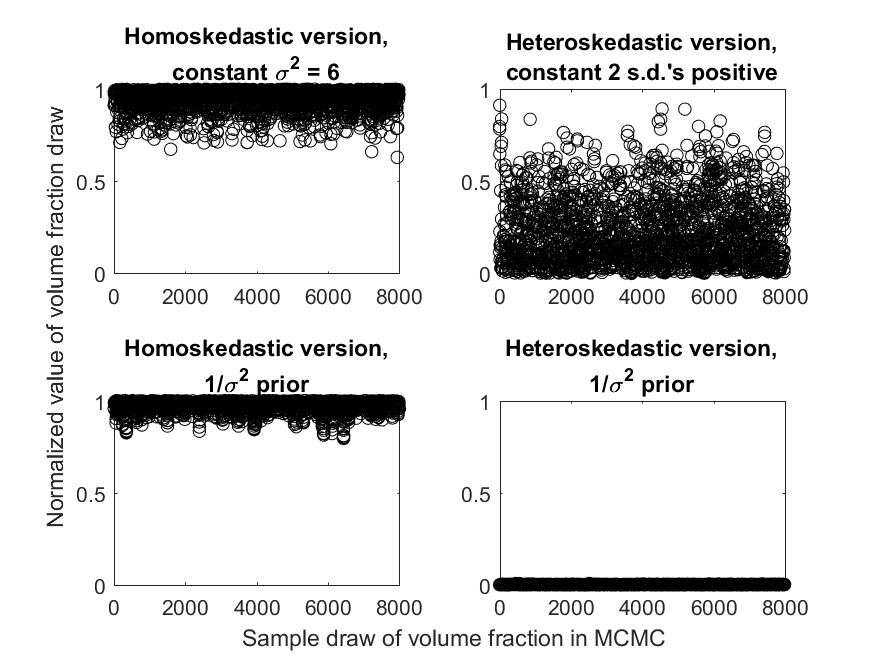
\includegraphics[width=.75\linewidth]{FIG_comp_obs_var}
%\captionsetup{width=.65\linewidth}
%\caption{MCMC results of volume fraction at various observation variance settings, on normalized scale. The heteroskedastic constant variance was chosen so that each of the three desired outputs is two standard deviations above zero; e.g., $\sigma^2_1 = \left(\frac12\cdot 0.65\right)^2\approx0.106$. The homoskedastic constant was set at 6 for each standardized output.}
%\label{fig:comp_obs_var}
%\end{figure}

%% USE scatterhist function -- not sure if this is the right location for it

%\subsection{Which targets to set?}\label{which_data}
%
%A related question to the setting of the observation variance of the desired observation is the setting of the desired observations themselves. I described some general considerations in Section \ref{level_of_desired_data} above, the upshot of which is that it is generally preferable to set desired observations as close to achievable as possible while remaining confident that the observations are not in fact realistically achievable. 
%
%In the case of heteroskedastic observation variance with a (non-degenerate) prior, the specific choice of desired data is not crucial. But where observation variance is either set to a known value or constrained to be equal (up to pre-specified scalar multiple) across outputs, the choice of desired data will matter for the same reason that the constraints on observation variance matter. To see this, consider performing the wind turbine blade calibration with observation variances set equal to $\sigma^2=6$ for all model outputs, where the desired deflection, rotation, and cost are set to $\mathbf d=[0.65,\ 0.077,\ 96]$. These values are the lower bounds on what is known to be plausible ranges for each output. The MCMC results for volume fraction draws and the resulting posterior mean model output for these settings are shown in Figure \ref{fig:comp_obs_var} and Table \ref{table:obs_vvar_comp}. Consider now replacing $\mathbf d$ with $\mathbf d'=[0.65,\ 0.077,\ -500]$. The effect of this would be equivalent to keeping $\mathbf d$ and reducing the observation variance for cost from 6 to a much lower value, insofar as each of these two changes amounts to increasing the Mahalanobis distance of each draw from the desired observation along the axis of cost. This, in turn, would have the effect in the calibration procedure of prioritizing cost at the expense of the performance metrics. Thus when one wishes to strike a balance of priorities in the calibration procedure, this will necessarily involve both constraints upon the observation variance and the choice of desired observations. A further illustration of the impact of this choice is in Table \ref{table:d_comp}, where two different levels of desired observations are compared under a pre-specified constant observation variance.
%
%Figure \ref{fig:des_data} illustrates the sort of difficulty that can arise if one fails to make one's desired observations sufficiently ambitious. Here, a separate $1/\sigma^2_i$ prior was placed on each of the three types of observation variance. The top set of plots show the MCMC results for an appropriately ambitious (i.e. not realistically achievable) desired observations (here rotation has been removed from the model for simplicity). The desired observations yield good mixing in the MCMC routine. In the bottom plots, the desired observation of deflection is still lower than what is realistically achievable, whereas the cost is low but achievable. The model can yield this desired cost, and so draws of the observation variance for cost quickly drift to extremely low values. As a result, the MCMC samples only from the very small region of the parameter space corresponding to cost very near \$163. The extremely strong correlation of VF and thickness within this region can be seen in the bottom right plot of Figure \ref{fig:des_data}. The small size of this region makes it difficult to sample from. But more importantly, samples from this region are not of particular interest, since it is possible to outperform this region in cost without sacrificing other desiderata. If one were antecedently unaware that this region can be outperformed, that fact would be suggested by the ability of the MCMC to find a region that meets the cost target (nearly) exactly without much variation in meeting the other desiderata. Indeed, this outcome of extremely low observation variance -- when observation variance is sampled under a prior -- serves as a way to detect that one's desired observation is in fact realistically achievable.
%
%When one \emph{knowingly} sets a realistically achievable outcome as a desired observation, it is preferable to specify a constant observation variance, or at least a lower bound on observation variance. In this way, one avoids the convergence difficulties of the lower plots in Figure \ref{fig:des_data}. In essence, setting a lower bound on the observation variance of cost would ``fatten'' the thin line of accepted draws represented in the rightmost plot, enhancing the ease with which the MCMC routine can explore the parameter space, and improving the acceptance ratio. However, where an analysis calls for strict adherence to a given target observation (so that such ``fattening'' is unpalatable), tools of low probability estimation can be brought to bear. Sequential Monte Carlo \citep{Doucet2001,Liu2001a} or subset simulation \citep{Au2001a,Au2003,Zuev2012a} can be used to sample from the low-probability space associated with a tight bound on a desired observation.
%%\subsubsection{Differing results}
%% for different desired data values
%\begin{table}[h]
%\centering
%\begin{tabular}{| c | c  | c  |  c | c  | c | c | c |}
%\hline
%Desired data $\mathbf d$ & $\sigma^2_{defl}$ & $\sigma^2_{rot}$ & $\sigma^2_{cost}$ & $\mu_{v|\mathbf d}$ &
%                            $\mu_{h|\mathbf d}$ & $\sigma^2_{v|\mathbf d}$ & $\sigma^2_{h|\mathbf d}$\\
%\hline
%$(0, 0, 0)$ & 375.45 & 277.69 & 2.62 & 0.215 & $4.01 \cdot 10^{-2}$&
%	$4.41\cdot 10^{-2}$ & $1.92 \cdot 10^{-3}$\\
%$(0.65, 0.077, 96)$ & 16.74 & 15.25 & $4.62 \cdot 10^{-7}$ &
%	$1.09 \cdot 10^{-3}$ & $3.36 \cdot10^{-4}$ &
%	$1.02 \cdot 10^{-5}$ & $9.97 \cdot 10^{-6}$\\
%\hline
%\end{tabular}
%\captionsetup{width=.95\linewidth}
%\caption{Comparison of results for two different (low) values of $\mathbf d$. Values listed are, respectively, the posterior means for the observation variance of each model output, posterior means for volume fraction ($v$) and thickness ($h$), and posterior variance of volume fraction and thickness. The differing results reflect different prioritizations of cost over performance metrics, since volume fraction correlates positively with cost and negatively with deflection and rotation.}
%\label{table:d_comp}
%\end{table}
%
%\begin{figure}
%\centering
%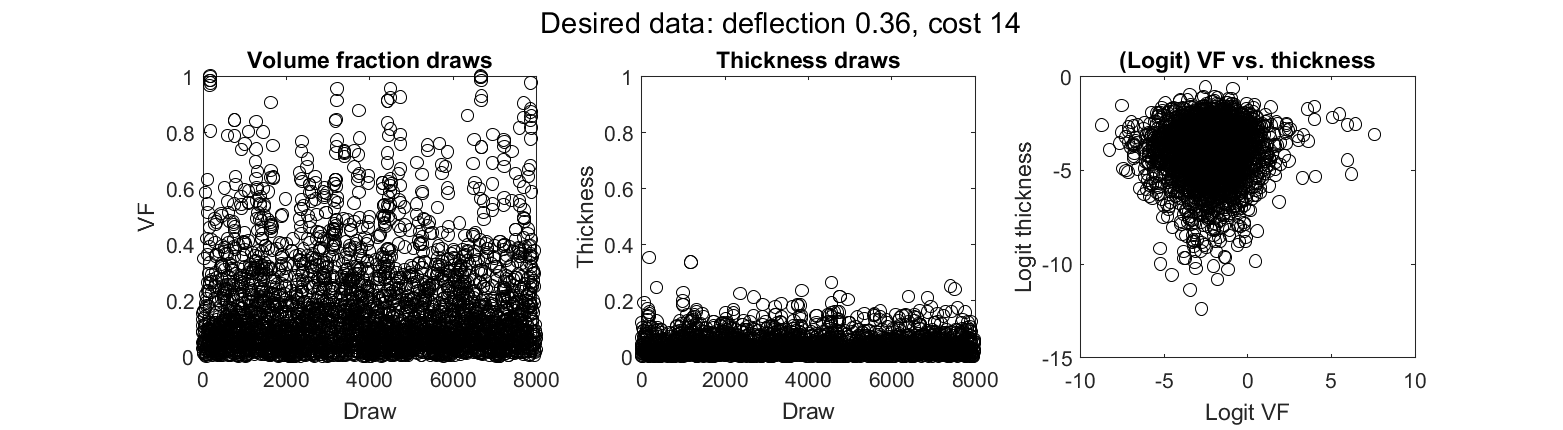
\includegraphics[width=.9\linewidth]{FIG1_posterior_samps_at_spec_cost}
%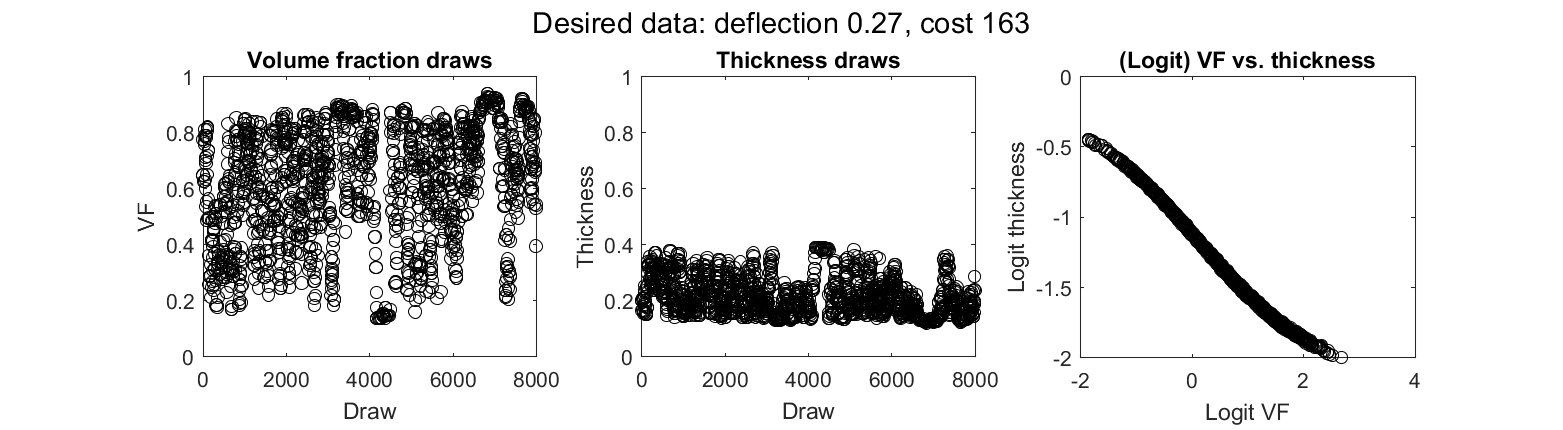
\includegraphics[width=.9\linewidth]{FIG2_posterior_samps_at_spec_cost}
%\captionsetup{width=.9\linewidth}
%\caption{MCMC results for low deflection and cost (top row) and low deflection with easily achievable cost (bottom row).}
%% NOTE: THESE PLOT TITLES ARE WRONG! GOTTA DO THE PLOTS OVER! LOL! but wait are they still
%\label{fig:des_data}
%\end{figure}

%\paragraph{Non-uniform prior on $\boldsymbol \theta$:}\label{non-uniform_prior}
%
%%\subsubsection{Implementation}
%
%The first option is attractive in those scenarios where one has rough knowledge of the correlation between the calibration parameters and a given model output. The strategy is to exploit this correlation to remove one of the desired observation outputs, where a prior is placed on the calibration parameters that is designed to control the removed model output.
%
%The wind turbine application serves as an example here. It is known that cost correlates strongly with each of the two calibration parameters (volume fraction $v$ and thickness $k$). Thus, I replace the uniform $\pi(\boldsymbol \theta)$ of (\ref{eq:the_model}) with a prior that penalizes high values of $v$ and $k$, thereby penalizing high cost output:
%\begin{equation}\label{eq:theta_prior}
%\pi(\boldsymbol \theta)=\pi(v,k)\propto \exp(-\lambda_{cost}\lVert (v,k)\rVert ^2)
%\end{equation}
%where $\lambda_{cost}$ can be set to any nonnegative value, with higher values resulting in stricter cost control. Pairing this with the $1/\sigma^2_i$ prior on observation variances, the full model becomes:
%\begin{equation}\label{full_model_3}
%\begin{aligned}
%\pi(\boldsymbol\theta,\mathbf C_{\mathbf y}|\mathcal D ) &\propto
%\pi(\mathcal D|\boldsymbol\theta,\mathbf C_{\mathbf y}) \times \pi(\boldsymbol\theta) \times \pi(\mathbf C_{\mathbf y})\\
%&\propto \lvert \mathbf C_{\mathcal D} \rvert ^{-1/2} \mathrm{exp}(\mathcal D^T \mathbf C_{\mathcal D}^{-1} \mathcal D) \times \mathrm{exp}(-\lambda_{cost}\lVert(v,k)\rVert^2)\times\prod_{i=1}^3 \frac1{\sigma^2_i}
%\end{aligned}
%\end{equation}
%
%This may seem to make little progress in resolving the complication of a model that includes cost, since now instead of specifying a desired cost we must specify a value for $\lambda_{cost}$. However, rather than specify a value for this hyperparameter, we can gain a more comprehensive picture of our options by observing the calibration results over a grid of values of $\lambda_{cost}$. Thus, rather than specifying beforehand what is our desired ``balance'' amongst cost, deflection and rotation, we are able to see a curve describing our options for this trade-off, and to then make an informed choice as to where on that curve we wish to be. 
%
%The decision-making value of such an analysis is further improved by including uncertainty quantification, which comes easily due to the nature of the Bayesian approach and GP emulator here. The draws of calibration parameters in the MCMC routine each correspond to a GP with posterior mean serving as an estimate of the true model output for those calibration settings. This captures the parameter uncertainty -- i.e., uncertainty remaining in the posterior distribution of the calibration parameters, which is uncertainty about which calibration parameter settings best achieve the desired observations. Furthermore, the GPs themselves are uncertain representations of the true model. For each draw of the calibration parameters in the MCMC routine, (\ref{posterior_GP}) gives us the mean and variance of the output at each control input. Thus we can use the posterior covariance of the GP to estimate the code uncertainty -- the uncertainty due to the variation of the GP around the true system mean. Thus a sort of ``Pareto band'' of model performance can guide decision-making in selecting a level for our calibration parameters. Decision-makers can observe surfaces describing the achievable system responses, with included uncertainty measures around those surfaces, and select a target outcome from this comprehensive picture of what is achievable. Figure \ref{fig:non-uniform_prior} gives an example of this for the wind turbine application. Figure \ref{fig:post_dists_lambda_cost} shows the posterior distributions of volume fraction and thickness for various values of $\lambda_{cost}$. 
%
%\begin{figure}
%\centering
%\captionsetup{width=.9\linewidth}
%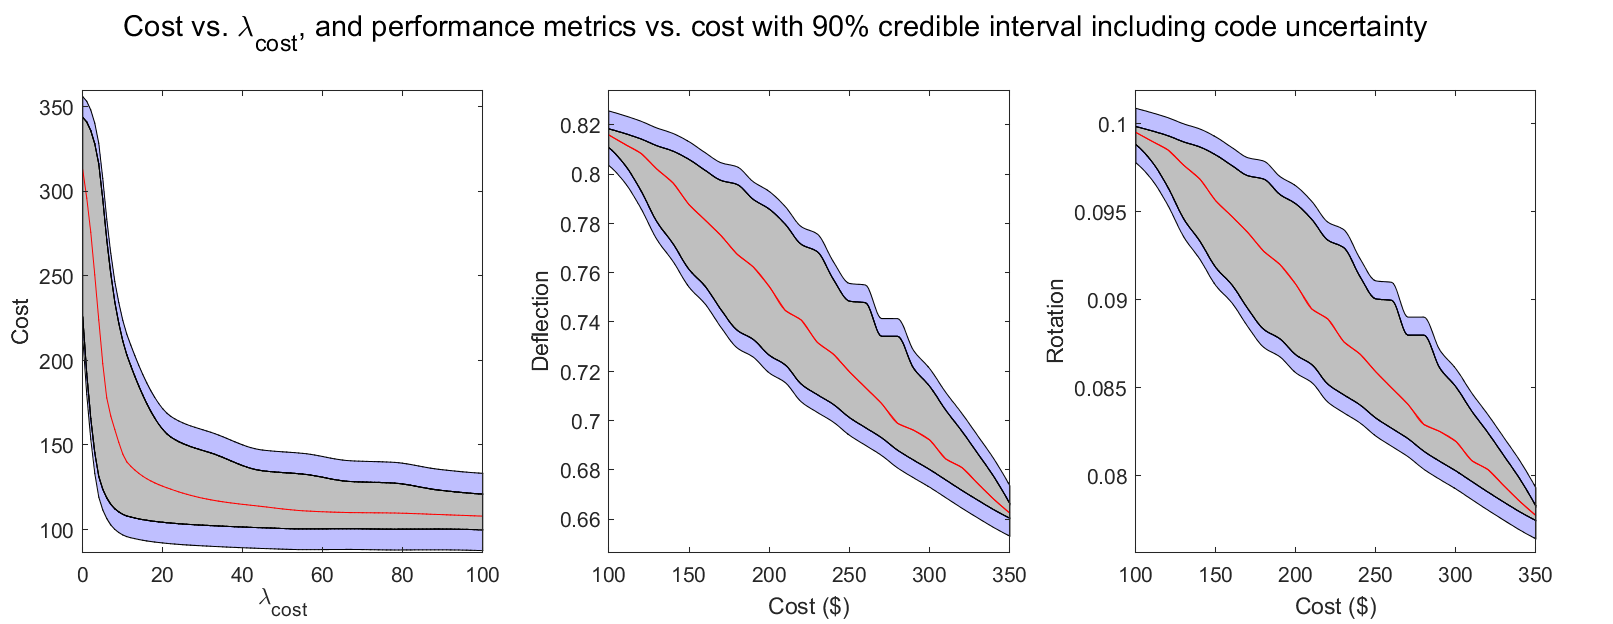
\includegraphics[width=\linewidth]{FIG_cost_lambda_code_uncert_upd}
%\caption{Resulting cost vs. $\lambda_{cost}$, and ``Pareto bands'' of wind turbine blade performance metric over a range of values of cost. Here, cost has been removed from the model and the prior $\exp(-\lambda_{cost}\lVert \theta \rVert^2)$ placed on the calibration parameters $\boldsymbol \theta$, with desired data 0 deflection and 0 rotation. The gray region gives a 90\% credible interval only considering parameter uncertainty. The blue region extends this to include code uncertainty, using the covariance of the posterior GPs corresponding to each draw of $\boldsymbol \theta$.}
%\label{fig:non-uniform_prior}
%\end{figure}
%
%
%\begin{figure}
%\centering
%\captionsetup{width=.7\linewidth}
%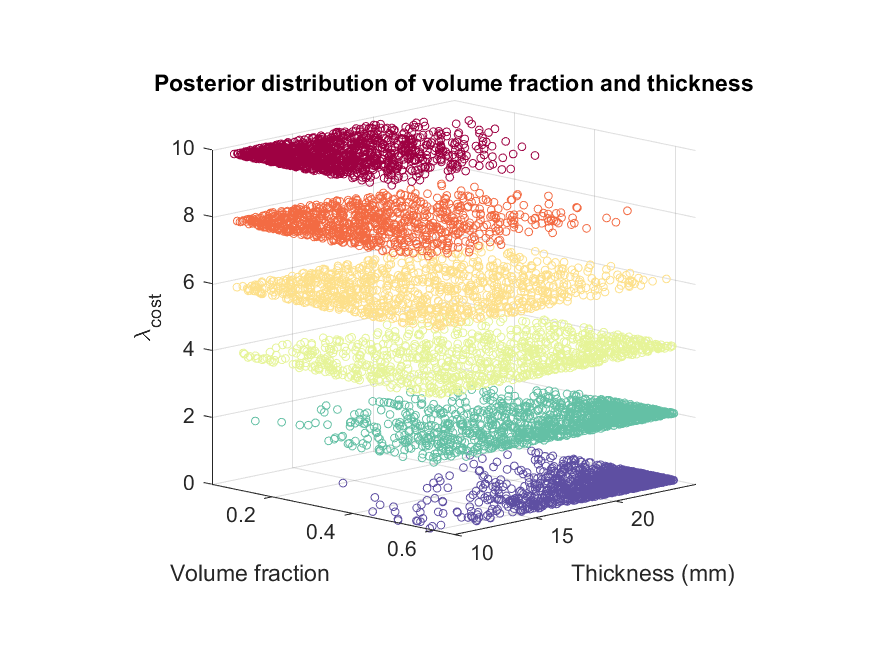
\includegraphics[width=.65\linewidth]{FIG_post_dist_across_cost_lambda-3d}
%\caption{Posterior distributions of volume fraction and thickness for various values of $\lambda_{cost}.$ Notice that higher values of $\lambda_{cost}$ push the distribution away from the (high-cost) upper region of the supports of the two variables.}
%\label{fig:post_dists_lambda_cost}
%\end{figure}

%\subsection{Exponentially distributed desired data}
%Blah

%\subsubsection{Motivation}
%Blah

%\subsubsection{Implementation and results}
%Blah


%\section{Future work}
%
%
%%\subsection{Alternative means of handling cost}
%%Blah
%
%%\subsubsection{Removing cost from the model}
%%Blah
%
%%\subsubsection{Alternative priors for controlling cost}
%%Blah
%
%%\subsection{Building a desired data response surface}
%%Blah
%
%\subsection{Hamiltonian Monte Carlo}
%
%Recall from Figure \ref{ACFs} that the autocorrelation in the MCMC routine, while much reduced by using the Metropolis-Hastings algorithm after applying a logit transformation to remove boundary conditions, is nonetheless still appreciable. In the application considered there, in order to achieve uncorrelated draws, one would save at most every $30^{\text{th} }$ draw. The efficiency of the algorithm can be improved by instead using the Hamiltonian Monte Carlo technique (HMC), also known as hybrid Monte Carlo \citep{Duane1987}. 
%
%Initially applied to lattice field theory simulations of quantum chromodynamics, HMC was popularized within the statistical community by \cite{Neal2011}. Neal describes the intuition supporting HMC roughly as follows. Consider the Metropolis-Hastings algorithm, in which a proposed new draw is drawn from a proposal distribution which is typically centered on the previous draw. Thus the position of the previous draw informs the next proposed draw. Rather than rely merely on the position of the previous draw, HMC relies both on its position and on its \emph{momentum}. The momentum of a variable moving in $p-$dimensional space can be understood on analogy to a puck moving on a horizontal two-dimensional surface curved in the third dimension to have areas of varying height. Negative likelihood for the variable is the analog for height. As the variable moves from an area of low likelihood to higher likelihood, it gains momentum, increasing the proposal density in the direction of that momentum. Likewise, as the variable moves from an area of high likelihood to low likelihood, its momentum can help carry it further into that space; but moving into the low likelihood space also reduces the variable's momentum, eventually causing the momentum to change direction.
%The result of these Hamiltonian dynamics in the sampling routine is to improve the efficiency of the exploration of the parameter space. Thus HMC works to reduce autocorellation beyond what is typically possible in Metropolis-Hastings. Therefore its use in the area of CDO can help to improve the efficiency of the sampling routine beyond what is seen in the righthand panel of Figure \ref{ACFs}.
%
%%\subsubsection{Hamiltonian Monte Carlo}
%% Background
%%Blah
%
%%\subsubsection{Benefits}
%%Blah
%
%\subsection{Model discrepancy}
%
%Recall from Section  \ref{model_shortcoming} that we may incorporate model shortcoming in two ways: as a form of observation variance, or as a form of model discrepancy. In Section \ref{MCMC}, observation variance serves as the basis for handling model shortcoming. This approach is attractive for its simplicity and for its flexibility in facilitating different calibration goals through modulation of the observation variances and their prior distributions. 
%However, as described in Section \ref{mod_disc}, there are advantages to using a model discrepancy $\delta(\cdot)$ instead of observation variance to incorporate model shortcoming. Most importantly, one's desired observation will tend to be systematically biased from the true system mean, and a model that incorporates shortcoming by way of Gaussian white noise, in an observation variance term, fails to capture this systematic bias. For this reason, future work in this area will include replacing observation variance with a prior mean-zero GP discrepancy function in the calibration procedure.
%
%Similarly, the technique of CDO as described in the present work assumes access to a computer model which is known to be accurate throughout the domain $\mathcal T$ over which the calibration occurs. Of course, in many applications, this assumption will not hold. Future extensions of the present work will include investigation of combining CDO with traditional calibration. This would be of interest in those situations where one has access to field observations and wishes to employ CDO. If computational expense makes simulation observations scarce, it will be particularly attractive to combine the two calibrations, using the same set of simulations for both calibrations simultaneously.
%
%I intend to pursue two avenues in this area. Firstly, one might capture model inadequacy with a traditional model discrepancy function, while simultaneously capturing model shortcoming via observation variance. In a full Bayesian analysis that treats desired observations as extra field observations, this would certainly lead to a lack of identifiability between the observation variance and the discrepancy function. However, the method of ``modularization'' \citep{Liu2009,Bayarri2007,Bayarri}, described above in Section \ref{computer_model_calibration}, can mitigate these difficulties, by partitioning the analysis so that desired observations do not bias the discrepancy function, and field observations do not bias the estimate of the observation variance of the desired observations.
%
%Secondly, one may attempt to capture model inadequacy and model shortcoming each in a separate discrepancy function. This will face the same difficulty as the first approach, and will likewise require modularization in order to retain the identifiability of the two discrepancy functions.
%
%\subsection{Comparison with optimization techniques}
%
%CDO is a form of optimization, and thus future work will include a thorough comparison of that approach to alternative forms of optimization. As well as comparing results, computational economy should be considered as a desideratum. Furthermore, CDO is a form of optimization under uncertainty, which can easily incorporate uncertainty in the model inputs, and which delivers a result which includes quantification of uncertainty on the posterior model outputs. Therefore, of particular interest are alternative means of optimization that accommodate and quantify uncertainty. \cite{Sahinidis2004} provides a useful overview of existing techniques for optimization under uncertainty; such techniques are the primary alternatives against which CDO should be considered.
%
%\section{Conclusion}
%% Discussion of the role of computer model validation as a potential methodology for design
%
%In this work I have described the theoretical background for the use of Gaussian processes to emulate computationally expensive computer model code, and the use of such emulators for computer model calibration under the framework established principally by \cite{Kennedy2001}, \cite{Williams2006} and \cite{Bayarri2007}. I have also described a modification of that framework which calibrates a computer model, not to field observations, but rather to desired observations, i.e., performance targets for the system. I described the implementation of this approach in an MCMC routine along with considerations to accommodate computational instability. I have also indicated future directions for research in the area of CDO.
%
%The use of this methodology is illustrated in the case of material design for a wind turbine blade. I have shown thereby a variety of ways in which CDO can be used to produce a guide that decision-makers can consult in the design process. By expropriating established tools of model calibration, CDO offers a method of optimization which is sensitive to all sources of uncertainty, and which results in an estimate that includes uncertainty quantification.
%
%
%\begin{appendices}
%
%\section{Full conditional distributions}
%Using a model that does not employ a discrepancy term, uses maximum likelihood estimation of $\boldsymbol \beta^\eta$ and $\lambda_\eta$, and sets the mean $c$ of the emulator to be 0, we have from \eqref{eq:full_dist} above that the joint posterior distribution is
%\begin{equation}
%\begin{aligned}
%\pi(\boldsymbol\theta,\mathbf C_{\mathbf y} | \mathcal D) &\propto
%\pi(\mathcal D|\boldsymbol\theta,\mathbf C_{\mathbf y}) \times \pi(\boldsymbol\theta) \times \pi(\mathbf C_{\mathbf y})\\
%&\propto \lvert \mathbf C_{\mathcal D} \rvert ^{-1/2} \exp (\mathcal D^T \mathbf C_{\mathcal D}^{-1}\mathcal D) \times \pi(\boldsymbol \theta) \times \pi(\mathbf C_{\mathbf y})
%\end{aligned}
%\end{equation}
%where $\mathbf C_{\mathcal D}$, given in \eqref{eq:C_D}, depends on both $\boldsymbol\theta$ and on $\mathbf C_{\mathbf y}$.
%Different priors on $\boldsymbol\theta$ and $\mathbf C_{\mathbf y}$ are used in the present work to flesh out this distribution. 
%For example, columns one and two of Table \ref{table:obs_vvar_comp} correspond to setting a uniform prior on $\boldsymbol\theta$ and specifying a set value for $\mathbf C_y$ (essentially thereby using a degenerate prior). 
%Thus over the support of $\boldsymbol \theta$ at the specified value of $\mathbf C_{\mathbf y}$, the joint posterior distribution is
%\begin{equation}\label{eq:fdupup}
%\begin{aligned}
%\lvert \mathbf C_{\mathcal D} \rvert ^{-1/2} \exp (\mathcal D^T \mathbf C_{\mathcal D}^{-1}\mathcal D) \times \pi(\boldsymbol \theta) \times \pi(\mathbf C_{\mathbf y}) &=\lvert \mathbf C_{\mathcal D} \rvert ^{-1/2} \exp (\mathcal D^T \mathbf C_{\mathcal D}^{-1}\mathcal D)
%\end{aligned}
%\end{equation}
%and since $\mathbf C_{\mathbf y}$ is specified in advance, this distribution is also the marginal posterior distribution of $\boldsymbol\theta$. 
%By contrast, columns three and four of Table \ref{table:obs_vvar_comp} place a reference prior on the observation variance of each model output. Recall that where $\sigma^2_i$ gives the observation variance for the $i^{th}$ model output, $\mathbf C_{\mathbf y}$ is a diagonal matrix with $i,i$ entry $\sigma^2_i$. 
%Column three of the table corresponds to a model in which each of the three outputs has its own observation variance, so that the prior $\pi(\mathbf C_{\mathbf y})=\prod_{i=1}^3 \sigma^{-2}_i$. 
%Column four uses a single observation variance for all three outputs, so that the prior is $\pi(\mathbf C_{\mathbf y})=\sigma^{-2}$. 
%Letting $K=3$ for column three and $K=1$ for column four, then, the joint posterior distribution is
%\begin{equation}\label{eq:fduprp}
%\begin{aligned}
%\lvert \mathbf C_{\mathcal D} \rvert ^{-1/2} \exp (\mathcal D^T \mathbf C_{\mathcal D}^{-1}\mathcal D) \times \pi(\boldsymbol \theta) \times \pi(\mathbf C_{\mathbf y}) 
%&\propto\lvert \mathbf C_{\mathcal D} \rvert ^{-1/2} \exp (\mathcal D^T \mathbf C_{\mathcal D}^{-1}\mathcal D) \times \prod_{i=1}^K \sigma^{-2}_i
%\end{aligned}
%\end{equation}
%where $\pi(\boldsymbol\theta)$ is again set to be uniform.
%Thus the posterior conditional distributions are
%\begin{equation}\label{eq:cduprp}
%\begin{aligned}
%\pi(\boldsymbol\theta|\mathbf C_{\mathbf y},\mathcal D) &\propto
%\lvert \mathbf C_{\mathcal D} \rvert ^{-1/2} \exp (\mathcal D^T \mathbf C_{\mathcal D}^{-1}\mathcal D) \\
%\pi(\mathbf C_{\mathbf y}| \boldsymbol \theta ,\mathcal D) &\propto
%\lvert \mathbf C_{\mathcal D} \rvert ^{-1/2} \exp (\mathcal D^T \mathbf C_{\mathcal D}^{-1}\mathcal D) \times \prod_{i=1}^K \sigma^{-2}_i.
%\end{aligned}
%\end{equation}
%
%Section \ref{removing_cal_pars} employs a model which places an informative prior on $\boldsymbol \theta$. A reference prior is also placed on the observation variance of each model output. The resulting posterior distribution is thus
%\begin{equation}\label{eq:fdifrp}
%\begin{aligned}
%\lvert \mathbf C_{\mathcal D} \rvert ^{-1/2} \exp (\mathcal D^T \mathbf C_{\mathcal D}^{-1}\mathcal D) \times \pi(\boldsymbol \theta) \times \pi(\mathbf C_{\mathbf y}) 
%&\propto\lvert \mathbf C_{\mathcal D} \rvert ^{-1/2} \exp (\mathcal D^T \mathbf C_{\mathcal D}^{-1}\mathcal D) \times 
%\exp(-\lambda_{cost} \lVert \boldsymbol\theta\rVert^2) \times
%\prod_{i=1}^3 \sigma^{-2}_i
%\end{aligned}
%\end{equation}
%and the posterior conditional distributions are given by
%\begin{equation}\label{eq:cdifrp}
%\begin{aligned}
%\pi(\boldsymbol\theta|\mathbf C_{\mathbf y},\mathcal D) 
%&\propto \lvert \mathbf C_{\mathcal D} \rvert ^{-1/2} \exp (\mathcal D^T \mathbf C_{\mathcal D}^{-1}\mathcal D) \times 
%\exp(-\lambda_{cost} \lVert \boldsymbol\theta\rVert^2)\\
%\pi(\mathbf C_{\mathbf y}| \boldsymbol \theta ,\mathcal D) &\propto
%\lvert \mathbf C_{\mathcal D} \rvert ^{-1/2} \exp (\mathcal D^T \mathbf C_{\mathcal D}^{-1}\mathcal D) \times 
%\prod_{i=1}^3 \sigma^{-2}_i.
%\end{aligned}
%\end{equation}
%%Notice that this model includes the model of \eqref{eq:fduprp} and \eqref{eq:cduprp} as a special case, by setting $\lambda_{cost}=0$.
%
%\section{Algorithm for MCMC}
%
%The following algorithm describes how to sample from the model given in \eqref{eq:fdifrp} and \eqref{eq:cdifrp}, which includes the model of \eqref{eq:fduprp} and \eqref{eq:cduprp} as a special case, by setting $\lambda_{cost}=0$. 
%Minor and straightforward modifications are required to sample from the model of \eqref{eq:fdupup}. In the algorithm, single-variable functions applied to multivariate input are applied componentwise; e.g., $\exp\left(\mathrm MVN([0, 0]^T,I_2)\right)$ denotes $[\exp(r_1), \exp(r_2)]$ where $[r_1, r_2]^T\sim\mathrm{MVN}([0, 0]^T,I_2)$.
%
%\begin{algorithm}
%%    \SetKwInOut{Input}{Input}
%%    \SetKwInOut{Output}{Output}
%%
%%    \underline{function Euclid} $(a,b)$\;
%%    \Input{Two nonnegative integers $a$ and $b$}
%%    \Output{$\gcd(a,b)$}
%%    \eIf{$b=0$}
%%      {
%%        return $a$\;
%%      }
%%      {
%%        return Euclid$(b,a\mod b)$\;
%%      }
%\textbf{Step 1:} Draw $\boldsymbol \theta^{(0)}\sim \mathrm {Unif}([0,1]^2)$, $(\sigma^2_j)^{(0)} \sim \mathrm {Gamma}(2,2)$ for $j=1,2,\ldots,K$. 
%Set $\mathbf C_{\mathbf y}$ using $(\sigma^2_j)^{(0)},\ j=1,2,\ldots,K$.
%Set $\mathbf C_{\mathcal D}$ using $\boldsymbol\theta^{(0)}$ and $\mathbf C_{\mathbf y}$.
%Specify $s^2=1$. 
%Specify $\lambda_{cost}\geq0$. Specify total number of iterations $M$ and burn-in $b$.
%Set $\mathrm{mult}=2$.
%Set $\Sigma=I_2$.
%Set $A=0$ and $A_\sigma=0$.
%Set $i=0$.
%
%\textbf{Step 2:} Repeat $M$ times.
%\begin{itemize}
%\item Update $i = i+1$.
%\item Draw $\boldsymbol \theta ^* \sim \mathrm{logit}^{-1}\left( \mathrm{MVN}(\mathrm{logit}(\boldsymbol \theta^{(i-1)}),\Sigma)\right)$.
%\item Set $\mathbf C_{\mathcal D}^*$ using $\boldsymbol\theta^*$ and $\mathbf C_{\mathbf y}$.
%\item Find 
%\begin{align*}
%\log \alpha = &
%\log \left( \lvert \mathbf C^*_{\mathcal D}\rvert^{-1/2} \exp(\mathcal D^T \mathbf {C_{\mathcal D}^*}^{-1}\mathcal D) \right) - 
%\lambda_{cost} \cdot \lVert \boldsymbol\theta^*\rVert^2 - 
%\log \left( \lvert \mathbf C_{\mathcal D}\rvert^{-1/2} \exp(\mathcal D^T \mathbf C_{\mathcal D}^{-1}\mathcal D) \right)  \\&+
%\lambda_{cost} \cdot \lVert \boldsymbol\theta^{(i-1)}\rVert^2 +
%\log \left ( \prod_{j=1}^2 \left( \theta^*_j(1-\theta_j^*) \right) \right ) - 
%\log \left (  \prod_{j=1}^2 \left( \theta^{(i-1)}_j(1-\theta_j^{(i-1)}) \right) \right )
%\end{align*}
%\item Draw $a\sim \mathrm{Unif}(0,1)$. If $a<\alpha$, set $\boldsymbol\theta^{(i)}=\boldsymbol\theta^*$, $\mathbf C_{\mathcal D} = \mathbf C_{\mathcal D}^*$, and increment $A=A+1$; otherwise, set $\boldsymbol\theta^{(i)} = \boldsymbol\theta^{(i-1)}$.
%\item Draw $[{\sigma_1^2}^*, {\sigma_2^2}^*, {\sigma_3^2}^*]^T \sim \exp \left ( \mathrm {MVN}\left( \log\left[{\sigma_1^2}^{(i-1)}, {\sigma_2^2}^{(i-1)}, {\sigma_3^2}^{(i-1)} \right]^T, s^2I_3 \right) \right)$.
%%\item Find $\log \alpha = \log \left( \lvert \mathbf C^*_{\mathcal D}\rvert^{-1/2} \exp(\mathcal D^T \mathbf {C_{\mathcal D}^*}^{-1}\mathcal D) \right) - \log\left(\prod_{j=1}^K {\sigma^2_k}^* \right)
%%- \log \left( \lvert \mathbf C_{\mathcal D}\rvert^{-1/2} \exp(\mathcal D^T \mathbf C_{\mathcal D}^{-1}\mathcal D) \right) + \log\left(\prod_{j=1}^K {\sigma^2_k}^{(i-1)} \right)
%%+ \log \left ( \prod_{j=1}^2 \left( \theta^*_j(1-\theta_j^*) \right) \right ) - \log \left (  \prod_{j=1}^2 \left( \theta^{(i-1)}_j(1-\theta_j^{(i-1)}) \right) \right )$.
%%\item Draw $\left[{\sigma^2_1}^*,{\sigma^2_2}^*,{\sigma^2_3}^*\right]^T\sim\exp\left ( \mathrm {MVN} \left ( \log \left[{\sigma^2_1}^{(i-1)},{\sigma^2_2}^{(i-1)},{\sigma^2_3}^{(i-1)}\right]^T,s^2I_3\right)\right) $
%\item Set $\mathbf C_{\mathbf y}^*$ using $\left[{\sigma^2_1}^*,{\sigma^2_2}^*,{\sigma^2_3}^*\right]^T$. Set $\mathbf C_{\mathcal D}^*$ using $\boldsymbol \theta^{(i)}$ and $\mathbf C_{\mathbf y}^*$.
%\item Find $\log \alpha = \log \left( \lvert \mathbf C^*_{\mathcal D}\rvert^{-1/2} \exp(\mathcal D^T \mathbf {C_{\mathcal D}^*}^{-1}\mathcal D) \right) - \log \left( \lvert \mathbf C_{\mathcal D}\rvert^{-1/2} \exp(\mathcal D^T \mathbf C_{\mathcal D}^{-1}\mathcal D) \right)$. 
%(Notice that the log ratio of priors $\log \left( \frac{\pi({\sigma^2_i}')}{\pi(\sigma^2_i)}\right)=\log \frac{{\sigma^2_i}}{{\sigma^2_i}'} = \log{\sigma^2_i}-\log{\sigma^2_i}'$ is cancelled out by the log Metropolis-Hastings correction for the asymetrical proposal density: $\log \left ( \frac{q(\sigma^2_i|{\sigma^2_i}')}{q({\sigma^2_i}'|\sigma^2_i)} \right)= \log\left( \frac{{\sigma^2_i}'}{\sigma^2_i} \right)= \log {\sigma^2_i}'- \log \sigma^2_i $.)
%\item Draw $a\sim \mathrm{Unif}(0,1)$. If $a<\alpha$, set $\left[{\sigma_1^2}^{(i)}, {\sigma_2^2}^{(i)}, {\sigma_3^2}^{(i)} \right]^T = \left[{\sigma_1^2}^{*}, {\sigma_2^2}^{*}, {\sigma_3^2}^{*} \right]^T$, $\mathbf C_{\mathbf y} = \mathbf C_{\mathbf y}^*$, $\mathbf C_{\mathcal D} = \mathbf C_{\mathcal D}^*$, and increment $A_\sigma = A_\sigma + 1$; otherwise, set $\left[{\sigma_1^2}^{(i)}, {\sigma_2^2}^{(i)}, {\sigma_3^2}^{(i)} \right]^T = \left[{\sigma_1^2}^{(i-1)}, {\sigma_2^2}^{(i-1)}, {\sigma_3^2}^{(i-1)} \right]^T$.
%\item If $i\leq b$ and $i\pmod {100} = 0$:
%\renewcommand{\labelitemii}{$\circ$}
%\begin{itemize}
%\item Update $\mathrm {mult} = 1.5 \cdot \mathrm{mult} \cdot \mathbf 1_{A>30} + 0.75 \cdot \mathrm {mult} \cdot \mathbf 1_{A<20}$. Set $A=0$.
%\item Update $\Sigma= \mathrm{mult} \cdot \mathrm {Cov}\left(\Theta\right)$, where $\Theta=\left[ {\boldsymbol\theta^{(1)}}, {\boldsymbol\theta^{(2)}}, \ldots, {\boldsymbol\theta^{(i)}} \right]^T$.
%\item Update $s^2 = 1.5 \cdot s^2 \cdot \mathbf 1_{A_\sigma>30} + 0.75 \cdot s^2 \cdot \mathbf 1_{A_\sigma<20}$. Set $A_\sigma=0$.
%\end{itemize}
%\end{itemize}
%    \caption{}
%\end{algorithm}
%
%
%
%
%\end{appendices}

